\chapter{Systematic construction of stabilizer codes via gauging abelian boundary symmetries}\label{app:codes}
\section{Synopsis}
In this project, we generalise a construction of the second author, published in ref.~\cite{GarreRubio2024}, to arbitrary spatial dimensions. Starting from a generic $d$-dimensional quantum state with an \emph{abelian} symmetry, we iteratively gauge the symmetry and its dual to obtain a state in one dimension higher. The admissible initial symmetries include global 0-form, higher-form, \emph{subsystem} and \emph{fractal symmetry}.

The resulting $(d+1)$-dimensional state naturally inherits this original symmetry at its boundary and can be shown to be the ground state of a local commuting projector Hamiltonian. The construction relies on an extension, developed in this work, of Williamson’s gauging procedure of \emph{submanifold symmetries}~\cite{Williamson2016b}. We formulate the framework in terms of tensor networks, where gauging maps are implemented as tensor network operators akin to those of ref.~\cite{Haegeman2014a}. The composition of these then provides a tensor network representation of the one-higher-dimensional state.

We illustrate the approach through several examples, including three-dimensional \emph{Clifford-deformed surface codes} and \emph{type-I fracton phases} obtained by gauging linear subsystem and \emph{Sierpinski} fractal symmetries.
\section{Reference}
\textit{Systematic construction of stabilizer codes via gauging abelian boundary symmetries} \par\noindent
\textbf{B. Vancraeynest-De Cuiper}, J. Garre-Rubio \par\noindent
\href{https:/doi.org/10.22331/q-2025-09-08-1852}{Quantum \textbf{9}, 1852 (2025)}, \href{https://doi.org/10.48550/arXiv.2410.09044}{arXiv:2410.09044}
\section{Contributions of the author}
%The current project is a generalisation of the construction developed in ref.~\cite{GarreRubio2024} by Jos\'e Garre-Rubio to arbitrary dimensions and general abelian symmetries. 

The main technical result underlying this project consists of a generalisation of the gauging procedure of Williamson, which in its original form was formulated for the symmetry group $\mbb Z_2$, to arbitrary abelian groups~\cite{Williamson2016b}. I derived this generalised gauging procedure and its associated dual symmetries conjointly with my co-author. The iterative gauging procedure is then obtained from this gauging procedure, the tensor network representation of which was constructed by me. I derived the introductory example of section 1, as well as the boundary conditions of the models appearing in sections 3 and 4. I wrote the majority of the manuscript.
%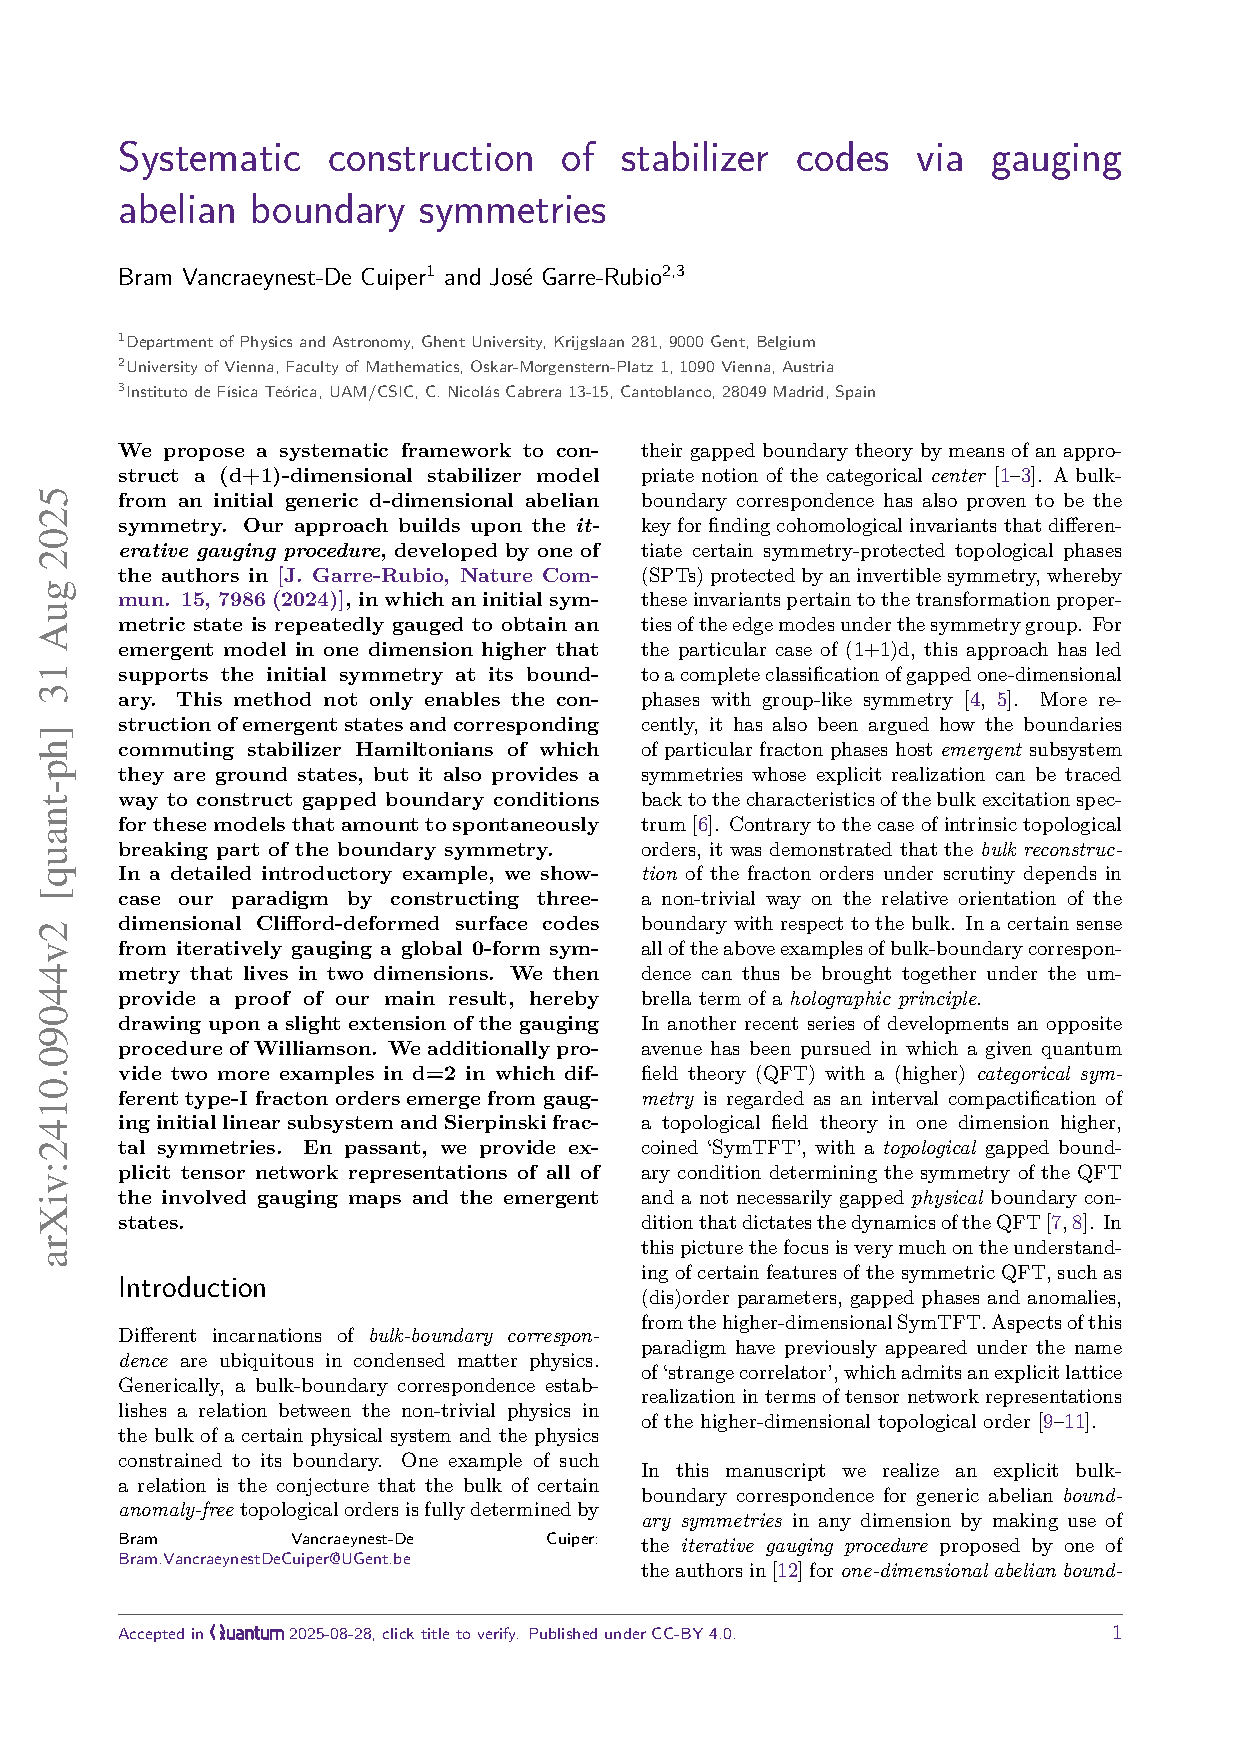
\includepdf[pages=-, trim=1.4cm 2.5cm 1.3cm 1cm, offset=-4mm 7mm, clip=true, frame=false, noautoscale=true, width=1.07\headwidth, pagecommand={}]{papers/stabilizers}
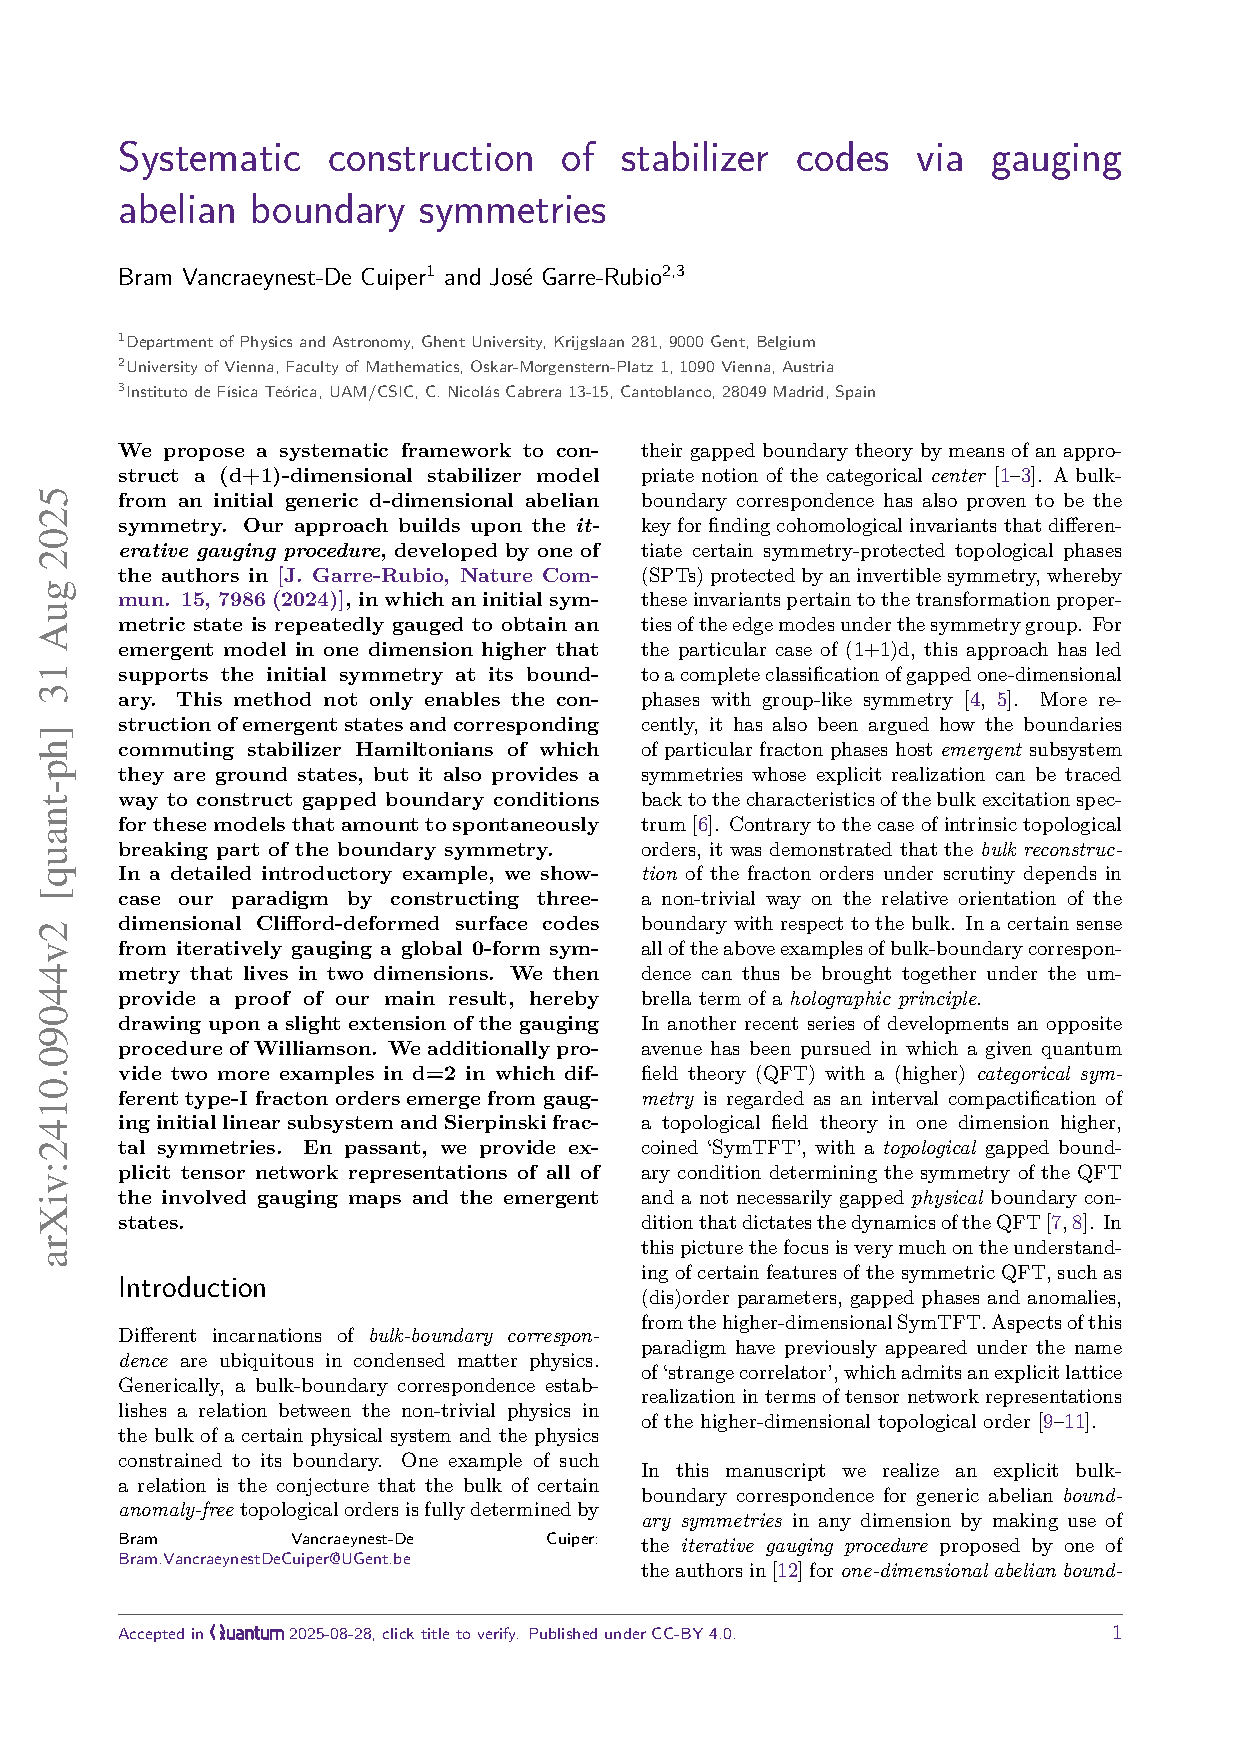
\includepdf[pages=-,
trim=17mm 27mm 17mm 17mm, clip=true,
noautoscale=true, width=\textwidth,
offset=-0.65mm 0mm,
pagecommand={\thispagestyle{publication}}]{papers/stabilizers}